% Usage: put \usepackage{graphicx} in the preamble, then include this file
% from the paperfuture project root. Adjust the asset path if moved.
\begin{figure*}[t]
  \centering
  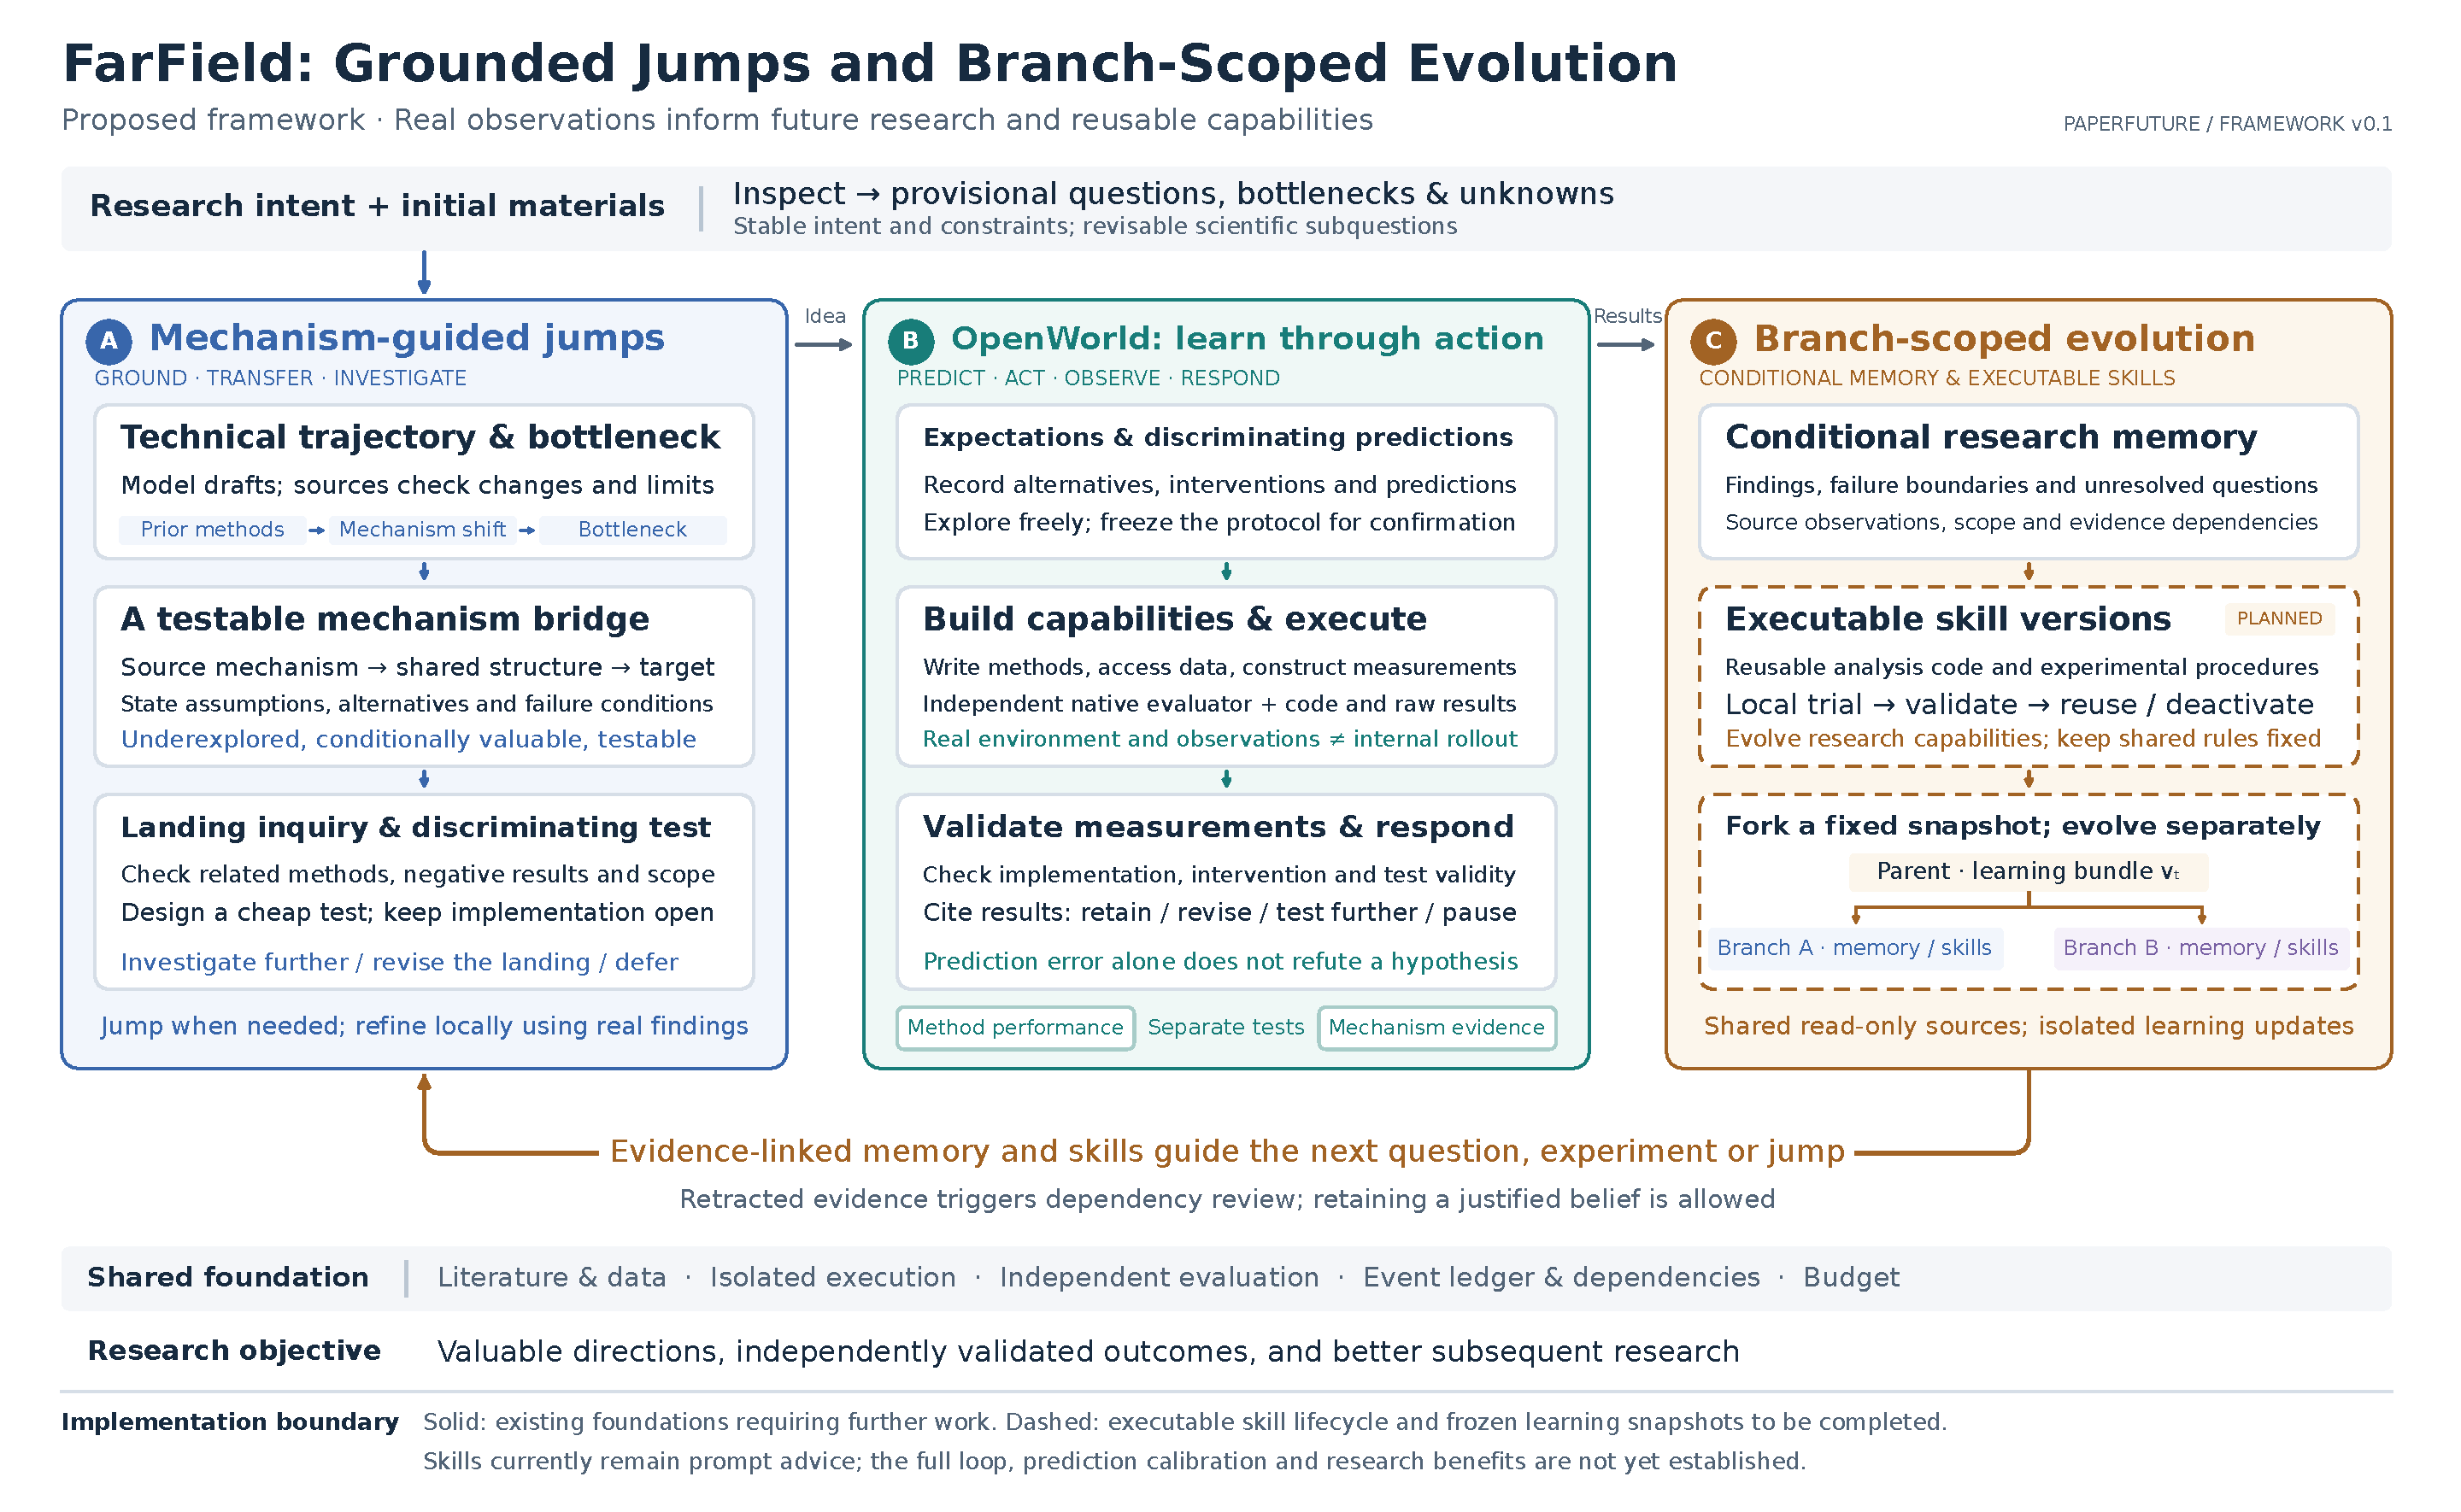
\includegraphics[width=\textwidth]{figures/farfield_framework_en.pdf}
  \caption{Proposed FarField research framework.
  (A) Mechanism-guided jumps connect a source mechanism to a target bottleneck
  through explicit assumptions, landing inquiry, and discriminating tests.
  (B) OpenWorld separates predictions from actual execution and requires
  evidence-based responses to observations; method performance and mechanism
  evidence are evaluated separately.
  (C) Branch-scoped learning links conditional memories and reusable skills to
  their source observations, with versioned inheritance and isolated updates.
  Learned capabilities inform subsequent questions, experiments, or jumps;
  each step need not invoke every component or perform a remote jump.
  Solid components have implementation foundations but remain incomplete;
  dashed components mark the proposed executable-skill lifecycle and fixed
  learning snapshots. The diagram describes the intended architecture and
  does not establish calibration, novelty, or research-performance gains.}
  \label{fig:farfield-framework}
\end{figure*}
